
\documentclass[tikz,border=10pt]{standalone}
\usepackage{tikz}
\usetikzlibrary{shapes.geometric, arrows.meta, positioning, fit, calc, backgrounds, shadows}

% Color Palette (Nature/Science style)
\definecolor{hmstBlue}{RGB}{66, 133, 244}   % Main Process
\definecolor{hmstRed}{RGB}{234, 67, 53}     % Controller/Decision
\definecolor{hmstGreen}{RGB}{52, 168, 83}   % Memory
\definecolor{hmstYellow}{RGB}{251, 188, 5}  % Warning/Critic
\definecolor{hmstGray}{RGB}{240, 240, 240}  % Backgrounds
\definecolor{darkGray}{RGB}{100, 100, 100}

\begin{document}

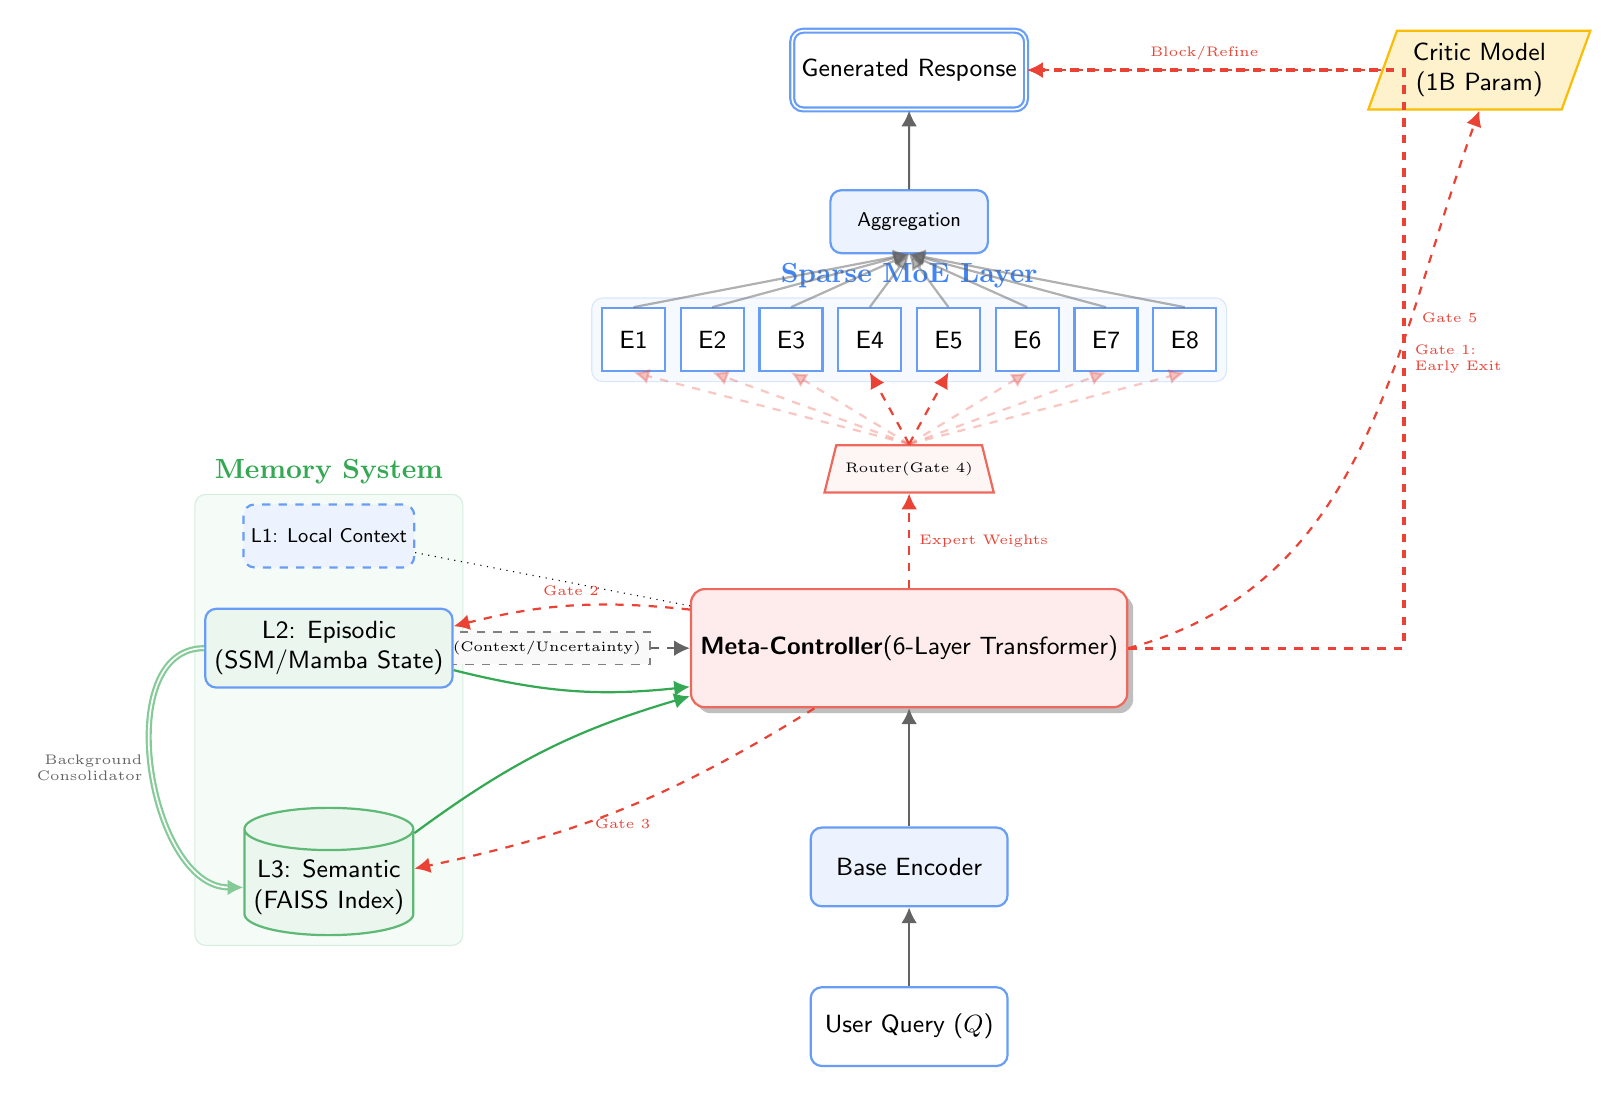
\begin{tikzpicture}[
    node distance=1.5cm and 2cm,
    font=\sffamily\small,
    >={Latex[width=2mm,length=2mm]},
    % Node Styles
    process/.style={
        rectangle,
        rounded corners,
        minimum width=2.5cm,
        minimum height=1cm,
        text centered,
        draw=hmstBlue!80,
        fill=hmstBlue!10,
        thick
    },
    controller/.style={
        rectangle,
        rounded corners=5pt,
        minimum width=3cm,
        minimum height=1.5cm,
        text centered,
        draw=hmstRed!80,
        fill=hmstRed!10,
        thick,
        drop shadow
    },
    memory/.style={
        cylinder,
        shape border rotate=90,
        aspect=0.25,
        minimum width=2cm,
        minimum height=1.5cm,
        text centered,
        draw=hmstGreen!80,
        fill=hmstGreen!10,
        thick
    },
    expert/.style={
        rectangle,
        minimum size=0.8cm,
        draw=hmstBlue!80,
        fill=white,
        thick
    },
    router/.style={
        trapezium,
        trapezium stretches body,
        trapezium angle=70,
        minimum width=1.5cm,
        minimum height=0.6cm,
        draw=hmstRed!80,
        fill=hmstRed!5,
        thick,
        font=\tiny
    },
    decision/.style={
        diamond,
        aspect=1.5,
        minimum width=1.5cm,
        draw=hmstRed!80,
        fill=white,
        font=\tiny
    },
    critic/.style={
        trapezium,
        trapezium left angle=70,
        trapezium right angle=110,
        minimum width=2.5cm,
        minimum height=1cm,
        draw=hmstYellow!100!orange,
        fill=hmstYellow!20,
        thick
    },
    state_summary/.style={
        rectangle,
        dashed,
        draw=gray,
        fill=gray!5,
        font=\tiny
    },
    % Connector Styles
    flow/.style={->, thick, darkGray},
    control/.style={->, thick, hmstRed, dashed},
    memory_link/.style={->, thick, hmstGreen},
    consolidation/.style={->, double, thick, hmstGreen!60}
]

% --- 1. Central Spine ---

% Input
\node (input) [process, fill=white] {User Query ($Q$)};

% Encoding
\node (encoder) [process, above=1cm of input] {Base Encoder};
\draw[flow] (input) -- (encoder);

% Meta-Controller
\node (meta) [controller, above=1.5cm of encoder] {\textbf{Meta-Controller}\\(6-Layer Transformer)};
\draw[flow] (encoder) -- (meta);

% State Summary Input
\node (state) [state_summary, left=0.5cm of meta] {State Summary\\(Context/Uncertainty)};
\draw[flow, dashed] (state) -- (meta);

% --- 2. Memory Hierarchy (Left Flank) ---

% L2 Episodic
\node (episodic) [process, left=3cm of meta, align=center, fill=hmstGreen!10] {L2: Episodic\\(SSM/Mamba State)};
\draw[control] (meta) to[bend right=10] node[midway, above, font=\tiny, text=hmstRed] {Gate 2} (episodic);
\draw[memory_link] (episodic) to[bend right=10] (meta);

% L3 Semantic
\node (semantic) [memory, below=1.5cm of episodic, align=center] {L3: Semantic\\(FAISS Index)};
\draw[control] (meta) to[bend left=10] node[midway, below, font=\tiny, text=hmstRed] {Gate 3} (semantic);
\draw[memory_link] (semantic) to[bend left=10] (meta);

% Consolidation Flow (outer left edge, asynchronous)
\draw[consolidation] (episodic.west) to[out=180, in=180] node[midway, left, font=\tiny, text=darkGray, align=right] {Background\\Consolidator} (semantic.west);

% L1 Attention (Implied/Small)
\node (l1) [process, above=0.5cm of episodic, scale=0.8, dashed] {L1: Local Context};
\draw[dotted] (l1) -- (meta);

% --- 3. Compute Layer (Top) ---

% Router Node (explicit decision point)
\node (router) [router, above=1.2cm of meta] {Router\\(Gate 4)};
\draw[control] (meta.north) -- node[midway, right, font=\tiny, text=hmstRed] {Expert Weights} (router.south);

% Experts Container
\node (moe_hub) [above=1.2cm of router] {};

% Draw 8 Experts
\foreach \i in {1,2,...,8} {
    \node (exp\i) [expert] at ($(moe_hub) + ({(\i-4.5)*1.0}, 0)$) {E\i};
}

% Routing Lines from Router to Experts
\draw[control] (router.north) -- (exp4.south);
\draw[control] (router.north) -- (exp5.south);
% Connect others lightly (inactive experts)
\foreach \i in {1,2,3,6,7,8} {
    \draw[control, opacity=0.3] (router.north) -- (exp\i.south);
}

% --- 4. Verification & Output (Right/Top) ---

% Aggregation
\coordinate (agg) at ($(moe_hub) + (0, 1.5)$);
\node (aggregate) [process, at=(agg), scale=0.8] {Aggregation};
\foreach \i in {1,...,8} {
    \draw[flow, opacity=0.5] (exp\i.north) -- (aggregate.south);
}

% Output
\node (output) [process, above=1cm of aggregate, fill=white, double] {Generated Response};
\draw[flow] (aggregate) -- (output);

% Critic (right side, moved further right for Early Exit clearance)
\node (critic) [critic, right=4.5cm of output, align=center] {Critic Model\\(1B Param)};
\draw[control] (meta.east) to[out=15, in=250] node[pos=0.7, right, font=\tiny, text=hmstRed] {Gate 5} (critic.south);
\draw[control, dashed] (critic.west) -- node[midway, above, font=\tiny] {Block/Refine} (output.east);

% Early Exit Path (vertical, far right, bypasses all computation)
\coordinate (early_exit_start) at ($(meta.east) + (3.5, 0)$);
\coordinate (early_exit_end) at ($(output.east) + (1.5, 0)$);
\draw[control, very thick] (meta.east) -- (early_exit_start) |- node[near start, right, font=\tiny, text=hmstRed, align=left] {Gate 1:\\Early Exit} (early_exit_end) -- (output.east);

% --- Backgrounds/Grouping ---

\begin{pgfonlayer}{background}
    % Memory Group
    \node [fit=(episodic) (semantic) (l1), fill=hmstGreen!5, rounded corners, draw=hmstGreen!20, label={[hmstGreen, font=\bfseries]above:Memory System}] {};

    % MoE Group
    \node [fit=(exp1) (exp8), fill=hmstBlue!5, rounded corners, draw=hmstBlue!20, label={[hmstBlue, font=\bfseries]above:Sparse MoE Layer}] {};
\end{pgfonlayer}

\end{tikzpicture}
\end{document}
